\section{Credentials Processes}
\url{https://docs.microsoft.com/en-us/windows-server/security/windows-authentication/credentials-processes-in-windows-authentication}

Windows credentials management is the process by which the operating system receives the credentials from the service or user and secures that information for future presentation to the authenticating target. In the case of a domain-joined computer, the authenticating target is the domain controller. The credentials used in authentication are digital documents that associate the user's identity to some form of proof of authenticity, such as a certificate, a password, or a PIN

By default, Windows credentials are validated against the Security Accounts Manager (SAM) database on the local computer, or against Active Directory on a domain-joined computer, through the Winlogon service. Credentials are collected through user input on the logon user interface or programmatically via the application programming interface (API) to be presented to the authenticating target.

Local security information is stored in the registry under
\verb+HKEY_LOCAL_MACHINE\SECURITY+. Stored information includes policy settings, default security values, and account information, such as cached logon credentials. A copy of the SAM database is also stored here, although it is write-protected.

The following diagram shows the components that are required and the paths that credentials take through the system to authenticate the user or process for a successful logon.

\begin{figure}
  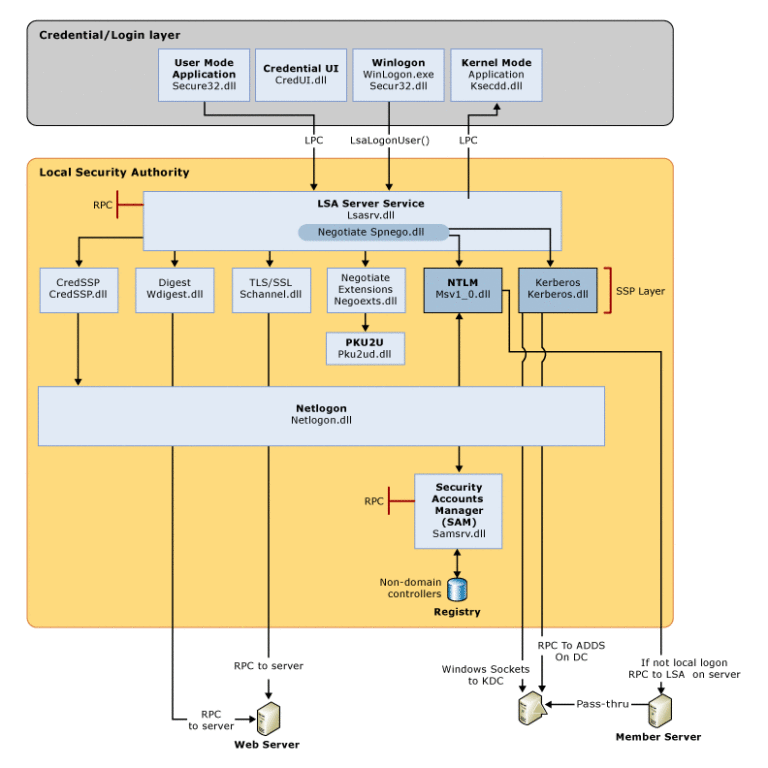
\includegraphics[width=\linewidth]{windows_knowledge/authentication/images/credential.png}
  \caption{Credential process architecture}
  \label{fig:credential-process-architecture}
\end{figure}


\begin{itemize}
\item User logon: Winlogon.exe is the executable file responsible for managing secure user interactions. The Winlogon service initiates the logon process for Windows operating systems by passing the credentials collected by user action on the secure desktop (Logon UI) to the Local Security Authority (LSA) through Secur32.dll
\item Application logon: Application or service logons that do not require interactive logon. Most processes initiated by the user run in user mode by using Secur32.dll whereas processes initiated at startup, such as services, run in kernel mode by using Ksecdd.sys.

For more information about user mode and kernel mode, see Applications and User Mode or Services and Kernel Mode in this topic.
\item Secur32.dll: The multiple authentication providers that form the foundation of the authentication process.
\item Lsasrv.dll: The LSA Server service, which both enforces security policies and acts as the security package manager for the LSA. The LSA contains the Negotiate function, which selects either the NTLM or Kerberos protocol after determining which protocol is to be successful.
\item Security Support Providers: A set of providers that can individually invoke one or more authentication protocols. The default set of providers can change with each version of the Windows operating system, and custom providers can be written.
\item Netlogon.dll: The services that the Net Logon service performs are as follows:
    \begin{itemize}
    \item  Maintains the computer's secure channel (not to be confused with Schannel) to a domain controller.
    \item Passes the user's credentials through a secure channel to the domain controller and returns the domain security identifiers (SIDs) and user rights for the user.
    \item Publishes service resource records in the Domain Name System (DNS) and uses DNS to resolve names to the Internet Protocol (IP) addresses of domain controllers.
    \item Implements the replication protocol based on remote procedure call (RPC) for synchronizing primary domain controllers (PDCs) and backup domain controllers (BDCs).
    \end{itemize}
\item Samsrv.dll: The Security Accounts Manager (SAM), which stores local security accounts, enforces locally stored policies and supports APIs.
\item Registry: The Registry contains a copy of the SAM database, local security policy settings, default security values, and account information that is only accessible to the system.
\end{itemize}

\subsection{Credential input for user logon}

In Windows Server 2008 and Windows Vista, the Graphical Identification and Authentication (GINA) architecture was replaced with a credential provider model, which made it possible to enumerate different logon types through the use of logon tiles. Both models are described below.

\subsubsection{Graphical Identification and Authentication architecture}

The Graphical Identification and Authentication (GINA) architecture applies to the Windows Server 2003, Microsoft Windows 2000 Server, Windows XP, and Windows 2000 Professional operating systems. In these systems, every interactive logon session creates a separate instance of the Winlogon service. The GINA architecture is loaded into the process space used by Winlogon, receives and processes the credentials, and makes the calls to the authentication interfaces through LSALogonUser.

The instances of Winlogon for an interactive logon run in Session 0. Session 0 hosts system services and other critical processes, including the Local Security Authority (LSA) process.

\subsubsection{Credential provider architecture}

the credentials input architecture changed to an extensible design by using credential providers. These providers are represented by the different logon tiles on the secure desktop that permit any number of logon scenarios - different accounts for the same user and different authentication methods, such as password, smart card, and biometrics.

With the credential provider architecture, Winlogon always starts Logon UI after it receives a secure attention sequence event. Logon UI queries each credential provider for the number of different credential types the provider is configured to enumerate. Credential providers have the option of specifying one of these tiles as the default. After all providers have enumerated their tiles, Logon UI displays them to the user. The user interacts with a tile to supply their credentials. Logon UI submits these credentials for authentication.

Credential providers are not enforcement mechanisms. They are used to gather
and serialize credentials. The \emph{Local Security Authority and
authentication packages enforce security}.

Credential providers are registered on the computer and are responsible for the following:
\begin{itemize}
    \item Describing the credential information required for authentication.

    \item Handling communication and logic with external authentication authorities.

    \item Packaging credentials for interactive and network logon.
\end{itemize}

Packaging credentials for interactive and network logon includes the process of serialization. By serializing credentials multiple logon tiles can be displayed on the logon UI. Therefore, your organization can control the logon display such as users, target systems for logon, pre-logon access to the network and workstation lock/unlock policies - through the use of customized credential providers. Multiple credential providers can co-exist on the same computer.


Single sign-on (SSO) providers can be developed as a standard credential provider or as a Pre-Logon-Access Provider.

Each version of Windows contains one default credential provider and one default Pre-Logon-Access Provider (PLAP), also known as the SSO provider. The SSO provider permits users to make a connection to a network before logging on to the local computer. When this provider is implemented, the provider does not enumerate tiles on Logon UI.

A SSO provider is intended to be used in the following scenarios:
\begin{itemize}
    \item  Network authentication and computer logon are handled by different credential providers. Variations to this scenario include:
    \begin{itemize}
        \item A user has the option of connecting to a network, such as connecting to a virtual private network (VPN), before logging on to the computer but is not required to make this connection.

        \item Network authentication is required to retrieve information used during interactive authentication on the local computer.

        \item Multiple network authentications are followed by one of the other scenarios. For example, a user authenticates to an Internet service provider (ISP), authenticates to a VPN, and then uses their user account credentials to log on locally.

        \item Cached credentials are disabled, and a Remote Access Services connection through VPN is required before local logon to authenticate the user.

        \item A domain user does not have a local account set up on a domain-joined computer and must establish a Remote Access Services connection through VPN connection before completing interactive logon.
    \end{itemize}
    \item Network authentication and computer logon are handled by the same credential provider. In this scenario, the user is required to connect to the network before logging on to the computer.
\end{itemize}

\subsubsection{Logon tile enumeration}
The credential provider enumerates logon tiles in the following instances:

\begin{itemize}
  \item  For those operating systems designated in the Applies to list at the beginning of this topic.

  \item  The credential provider enumerates the tiles for workstation logon. The credential provider typically serializes credentials for authentication to the local security authority. This process displays tiles specific for each user and specific to each user's target systems.

  \item  The logon and authentication architecture lets a user use tiles enumerated by the credential provider to unlock a workstation. Typically, the currently logged-on user is the default tile, but if more than one user is logged on, numerous tiles are displayed.

  \item  The credential provider enumerates tiles in response to a user request to change their password or other private information, such as a PIN. Typically, the currently logged-on user is the default tile; however, if more than one user is logged on, numerous tiles are displayed.

 \item   The credential provider enumerates tiles based on the serialized credentials to be used for authentication on remote computers. Credential UI does not use the same instance of the provider as the Logon UI, Unlock Workstation, or Change Password. Therefore, state information cannot be maintained in the provider between instances of Credential UI. This structure results in one tile for each remote computer logon, assuming the credentials have been correctly serialized. This scenario is also used in User Account Control (UAC), which can help prevent unauthorized changes to a computer by prompting the user for permission or an administrator password before permitting actions that could potentially affect the computer's operation or that could change settings that affect other users of the computer.
\end{itemize}

The following diagram shows the credential process for the operating systems designated in the Applies To list at the beginning of this topic.

\begin{figure}
  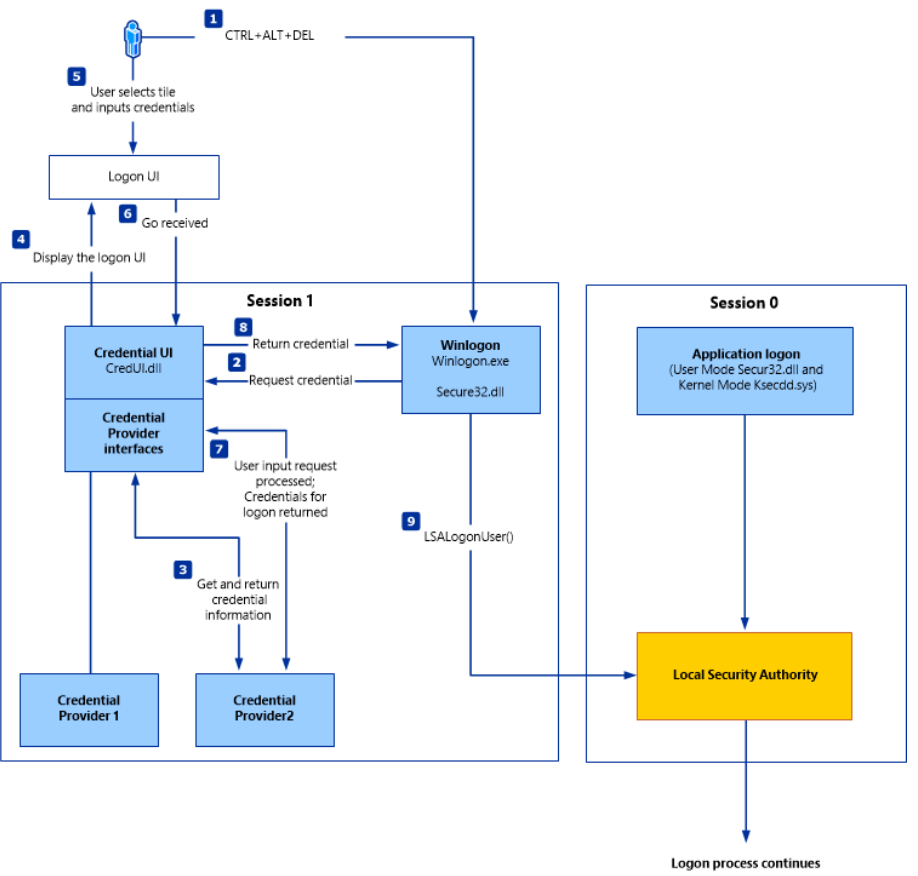
\includegraphics[width=\linewidth]{windows_knowledge/authentication/images/cred-input.png}
  \caption{Credential Input Process}
  \label{fig:credential-input-architecture}
\end{figure}


\subsection{Credential input for application and service logon}

Windows authentication is designed to manage credentials for applications or
services that do not require user interaction. Applications in user mode are
limited in terms of what system resources they have access to, while services
can have unrestricted access to the system memory and external devices.

System services and transport-level applications access an Security Support
Provider (SSP) through the Security Support Provider Interface (SSPI) in
Windows, which provides functions for enumerating the security packages
available on a system, selecting a package, and using that package to obtain an
authenticated connection.

When a client/server connection is authenticated:
\begin{itemize}
        \item The application on the client side of the connection sends
            credentials to the server by using the SSPI function
            \verb+InitializeSecurityContext+ (General).
        \item The application on the server side of the connection responds
            with the SSPI function \verb+AcceptSecurityContext+ (General).
        \item The SSPI functions \verb+InitializeSecurityContext+ (General) and
            \verb+AcceptSecurityContext+ (General) are repeated until all the
            necessary authentication messages have been exchanged to either
            succeed or fail authentication.
        \item After the connection has been authenticated, the LSA on the
            server uses information from the client to build the security
            context~\ref{win:security-context}, which contains an access
            token~\ref{win:access-token}.
        \item The server can then call the SSPI function
            \verb+ImpersonateSecurityContext+ to attach the access token to an
            impersonation thread for the service.
\end{itemize}

\subsubsection{Applications and user mode}

User mode in Windows is composed of two systems capable of passing I/O requests
to the appropriate kernel-mode drivers: the environment system, which runs
applications written for many different types of operating systems, and the
integral system, which operates system-specific functions on behalf of the
environment system.

The integral system manages operating system'specific functions on behalf of
the environment system and consists of a security system process (the LSA), a
workstation service, and a server service. The security system process deals
with security tokens, grants or denies permissions to access user accounts
based on resource permissions, handles logon requests and initiates logon
authentication, and determines which system resources the operating system
needs to audit.

Applications can run in user mode where the application can run as any
principal, including in the security context of \emph{Local System}
(\verb+SYSTEM+). Applications can also run in kernel mode where the application
can run in the security context of Local System (SYSTEM).

SSPI is available through the \verb+Secur32.dll+ module, which is an API used
for obtaining integrated security services for authentication, message
integrity, and message privacy. It provides an abstraction layer between
application-level protocols and security protocols. Because different
applications require different ways of identifying or authenticating users and
different ways of encrypting data as it travels across a network, SSPI provides
a way to access dynamic-link libraries (DLLs) that contain different
authentication and cryptographic functions. These DLLs are called Security
Support Providers (SSPs).


Managed service accounts and virtual accounts were introduced in Windows Server
2008 R2 and Windows 7 to provide crucial applications, such as Microsoft SQL
Server and Internet Information Services (IIS), with the isolation of their own
domain accounts, while eliminating the need for an administrator to manually
administer the service principal name (SPN) and credentials for these accounts.
For more information about these features and their role in authentication, see
Managed Service Accounts Documentation for Windows 7 and Windows Server 2008 R2
and Group Managed Service Accounts Overview.

\subsubsection{Services and kernel mode}

Even though most Windows applications run in the security context of the user
who starts them, this is not true of services. Many Windows services, such as
network and printing services, are started by the service controller when the
user starts the computer. These services might run as Local Service or Local
System and might continue to run after the last human user logs off.

{\bf Note}: Services normally run in security contexts known as Local System (SYSTEM), Network Service, or Local Service. Windows Server 2008 R2 introduced services that run under a managed service account, which are domain principals.

Before starting a service, the service controller logs on by using the account
that is designated for the service, and then presents the service's credentials
for authentication by the LSA. The Windows service implements a programmatic
interface that the service controller manager can use to control the service. A
Windows service can be started automatically when the system is started or
manually with a service control program. For example, when a Windows client
computer joins a domain, the messenger service on the computer connects to a
domain controller and opens a secure channel to it. To obtain an authenticated
connection, the service must have credentials that the remote computer's Local
Security Authority (LSA) trusts. When communicating with other computers in the
network, LSA uses the credentials for the local computer's domain account, as
do all other services running in the security context of the Local System and
Network Service. Services on the local computer run as SYSTEM so credentials do
not need to be presented to the LSA.

The file \verb+Ksecdd.sys+ manages and encrypts these credentials and uses a
local procedure call into the LSA. The file type is DRV (driver) and is known
as the kernel-mode Security Support Provider (SSP) and, in those versions
designated in the Applies To list at the beginning of this topic, is FIPS 140-2
Level 1-compliant.

Kernel mode has full access to the hardware and system resources of the
computer. The kernel mode stops user-mode services and applications from
accessing critical areas of the operating system that they should not have
access to.


\subsection{Local Security Authority}
\index{Windows:Local Security Authority}
\label{windows:lsa}

The \emph{Local Security Authority} (LSA) is a protected subsystem that
authenticates and signs in users to the local computer. In addition, LSA
maintains information about all aspects of local security on a computer (these
aspects are collectively known as the \emph{local security policy}). 

It also provides various services for translation between names and
\emph{security identifiers} (SIDs).

It keeps track of the security policies and the accounts that are in effect on a computer system.

It validates a user's identity based on which of the following two entities issued the user's account:

\begin{itemize}
    \item {\bf Local Security Authority}. The LSA can validate user information
        by checking the Security Accounts Manager (SAM) database located on the
        same computer. Any workstation or member server can store local user
        accounts and information about local groups. However, these accounts
        can be used for accessing only that workstation or computer.
    \item {\bf Security authority for the local domain or for a trusted
        domain}. The LSA contacts the entity that issued the account and
        requests verification that the account is valid and that the request
        originated from the account holder.
\end{itemize} 

\emph{Local Security Authority Subsystem Service} (LSASS) stores credentials in
memory on behalf of users with active Windows sessions. The stored credentials
let users seamlessly access network resources, such as file shares, Exchange
Server mailboxes, and SharePoint sites, without re-entering their credentials
for each remote service. Credentials are stored in multiple forms, including:


\begin{itemize}
    \item Reversibly encrypted plaintext
    \item Kerberos tickets (ticket-granting tickets (TGTs), service tickets)
    \item NT hash
    \item LAN Manager (LM) hash
\end{itemize}

If the user logs on to Windows by using a smart card, LSASS does not store a plaintext password, but it stores the corresponding NT hash value for the account and the plaintext PIN for the smart card. If the account attribute is enabled for a smart card that is required for interactive logon, a random NT hash value is automatically generated for the account instead of the original password hash. The password hash that is automatically generated when the attribute is set does not change.

If a user logs on to a Windows-based computer with a password that is compatible with LAN Manager (LM) hashes, this authenticator is present in memory.

The storage of plaintext credentials in memory cannot be disabled, even if the credential providers that require them are disabled.

The stored credentials are directly associated with the Local Security Authority Subsystem Service (LSASS) logon sessions that have been started after the last restart and have not been closed. For example, LSA sessions with stored LSA credentials are created when a user does any of the following:
\begin{itemize}
    \item Logs on to a local session or Remote Desktop Protocol (RDP) session on the computer
    \item Runs a task by using the RunAs option
    \item Runs an active Windows service on the computer
    \item Runs a scheduled task or batch job
    \item Runs a task on the local computer by using a remote administration tool
\end{itemize}

In some circumstances, the LSA secrets, which are secret pieces of data that are accessible only to SYSTEM account processes, are stored on the hard disk drive. Some of these secrets are credentials that must persist after reboot, and they are stored in encrypted form on the hard disk drive. Credentials stored as LSA secrets might include:
\begin{itemize}
    \item Account password for the computer's Active Directory Domain Services (AD DS) account
    \item Account passwords for Windows services that are configured on the computer
    \item Account passwords for configured scheduled tasks
    \item Account passwords for IIS application pools and websites
    \item Passwords for Microsoft accounts
\end{itemize}

Introduced in Windows 8.1, the client operating system provides additional protection for the LSA to prevent reading memory and code injection by non-protected processes. This protection increases security for the credentials that the LSA stores and manages.

For more information about these additional protections, see \href{https://docs.microsoft.com/en-us/windows-server/security/credentials-protection-and-management/configuring-additional-lsa-protection}{Configuring Additional LSA Protection}.

\subsection{Cached credentials and validation}
Validation mechanisms rely on the presentation of credentials at the time of
logon. However, when the computer is disconnected from a domain controller, and
the user is presenting domain credentials, Windows uses the process of cached
credentials in the validation mechanism.

Each time a user logs on to a domain, Windows caches the credentials supplied
and stores them in the security hive in the registry of the operation system.

With cached credentials, the user can log on to a domain member without being
connected to a domain controller within that domain.


\subsection{Credential storage and validation}
It is not always desirable to use one set of credentials for access to
different resources. For example, an administrator might want to use
administrative rather than user credentials when accessing a remote server.
Similarly, if a user accesses external resources, such as a bank account, he or
she can only use credentials that are different than their domain credentials.
The following sections describe the differences in credential management
between current versions of Windows operating systems and the Windows Vista and
Windows XP operating systems.

\subsubsection{Remote logon credential processes}
The Remote Desktop Protocol (RDP) manages the credentials of the user who
connects to a remote computer by using the Remote Desktop Client, which was
introduced in Windows 8. The credentials in plaintext form are sent to the
target host where the host attempts to perform the authentication process, and,
if successful, connects the user to allowed resources. RDP does not store the
credentials on the client, but the user's domain credentials are stored in the
LSASS.

Introduced in Windows Server 2012 R2 and Windows 8.1, Restricted Admin mode
provides additional security to remote logon scenarios. This mode of Remote
Desktop causes the client application to perform a network logon
challenge-response with the NT one-way function (NTOWF) or use a Kerberos
service ticket when authenticating to the remote host. After the administrator
is authenticated, the administrator does not have the respective account
credentials in LSASS because they were not supplied to the remote host.
Instead, the administrator has the computer account credentials for the
session. Administrator credentials are not supplied to the remote host, so
actions are performed as the computer account. Resources are also limited to
the computer account, and the administrator cannot access resources with his
own account.


\subsubsection{Automatic restart sign-on credential process}
When a user signs in on a Windows 8.1 device, LSA saves the user credentials in
encrypted memory that are accessible only by LSASS.exe. When Windows Update
initiates an automatic restart without user presence, these credentials are
used to configure Autologon for the user.

On restart, the user is automatically signed in via the Autologon mechanism,
and then the computer is additionally locked to protect the user's session. The
locking is initiated through Winlogon whereas the credential management is done
by LSA. By automatically signing in and locking the user's session on the
console, the user's lock screen applications is restarted and available.

For more information about ARSO, see 
\href{https://docs.microsoft.com/en-us/windows-server/security/windows-authentication/winlogon-automatic-restart-sign-on-arso}{Winlogon
Automatic Restart Sign-On (ARSO)}.

\subsubsection{Stored user names and passwords in Windows Vista and Windows XP}
In Windows Server 2008 , Windows Server 2003, Windows Vista, and Windows XP,
Stored User Names and Passwords in Control Panel simplifies the management and
use of multiple sets of logon credentials, including X.509 certificates used
with smart cards and Windows Live credentials (now called Microsoft account).
The credentials - part of the user's profile - are stored until needed. This
action can increase security on a per-resource basis by ensuring that if one
password is compromised, it does not compromise all security.

After a user logs on and attempts to access additional password-protected
resources, such as a share on a server, and if the user's default logon
credentials are not sufficient to gain access, Stored User Names and Passwords
is queried. If alternate credentials with the correct logon information have
been saved in Stored User Names and Passwords, these credentials are used to
gain access. Otherwise, the user is prompted to supply new credentials, which
can then be saved for reuse, either later in the logon session or during a
subsequent session.

The following restrictions apply:
\begin{itemize}
    \item If Stored User Names and Passwords contains invalid or incorrect
        credentials for a specific resource, access to the resource is denied,
        and the Stored User Names and Passwords dialog box does not appear.

    \item Stored User Names and Passwords stores credentials only for NTLM,
        Kerberos protocol, Microsoft account (formerly Windows Live ID), and
        Secure Sockets Layer (SSL) authentication. Some versions of Internet
        Explorer maintain their own cache for basic authentication.
\end{itemize}

These credentials become an encrypted part of a user's local profile in the
\verb+\Documents and Settings\Username\Application Data\Microsoft\Credentials+
directory. As a result, these credentials can roam with the user if the user's
network policy supports Roaming User Profiles. However, if the user has copies
of Stored User Names and Passwords on two different computers and changes the
credentials that are associated with the resource on one of these computers,
the change is not propagated to Stored User Names and Passwords on the second
computer.

\subsubsection{Windows Vault and Credential Manager}

Credential Manager was introduced in Windows Server 2008 R2 and Windows 7 as a
Control Panel feature to store and manage user names and passwords. Credential
Manager lets users store credentials relevant to other systems and websites in
the secure Windows Vault. Some versions of Internet Explorer use this feature
for authentication to websites.

Credential management by using Credential Manager is controlled by the user on
the local computer. Users can save and store credentials from supported
browsers and Windows applications to make it convenient when they need to sign
in to these resources. Credentials are saved in special encrypted folders on
the computer under the user's profile. Applications that support this feature
(through the use of the Credential Manager APIs), such as web browsers and
apps, can present the correct credentials to other computers and websites
during the logon process.

When a website, an application, or another computer requests authentication
through NTLM or the Kerberos protocol, a dialog box appears in which you select
the Update Default Credentials or Save Password check box. This dialog box that
lets a user save credentials locally is generated by an application that
supports the Credential Manager APIs. If the user selects the Save Password
check box, Credential Manager keeps track of the user's user name, password,
and related information for the authentication service that is in use.

The next time the service is used, Credential Manager automatically supplies
the credential that is stored in the Windows Vault. If it is not accepted, the
user is prompted for the correct access information. If access is granted with
the new credentials, Credential Manager overwrites the previous credential with
the new one and then stores the new credential in the Windows Vault.

\subsection{Security Accounts Manager (SAM)}
\index{Windows:Security Account Manager}
\label{win:SAM}
The Security Accounts Manager (SAM) is a database that stores local user
accounts and groups. It is present in every Windows operating system; however,
when a computer is joined to a domain, Active Directory manages domain accounts
in Active Directory domains.

For example, client computers running a Windows operating system participate in
a network domain by communicating with a domain controller even when no human
user is logged on. To initiate communications, the computer must have an active
account in the domain. Before accepting communications from the computer, the
LSA on the domain controller authenticates the computer's identity and then
constructs the computer's security context just as it does for a human security
principal. This security context defines the identity and capabilities of a
user or service on a particular computer or a user, service, or computer on a
network. For example, the access token contained within the security context
defines the resources (such as a file share or printer) that can be accessed
and the actions (such as Read, Write, or Modify) that can be performed by that
principal - a user, computer, or service on that resource.

The security context of a user or computer can vary from one computer to
another, such as when a user logs on to a server or a workstation other than
the user's own primary workstation. It can also vary from one session to
another, such as when an administrator modifies the user's rights and
permissions. In addition, the security context is usually different when a user
or computer is operating on a stand-alone basis, in a network, or as part of an
Active Directory domain.

\subsection{Local domains and trusted domains}
When a trust exists between two domains, the authentication mechanisms for each
domain rely on the validity of the authentications coming from the other
domain. Trusts help to provide controlled access to shared resources in a
resource domain (the trusting domain) by verifying that incoming authentication
requests come from a trusted authority (the trusted domain). In this way,
trusts act as bridges that let only validated authentication requests travel
between domains.a

How a specific trust passes authentication requests depends on how it is
configured. Trust relationships can be one-way, by providing access from the
trusted domain to resources in the trusting domain, or two-way, by providing
access from each domain to resources in the other domain. Trusts are also
either nontransitive, in which case a trust exists only between the two trust
partner domains, or transitive, in which case a trust automatically extends to
any other domains that either of the partners trusts.

For information about domain and forest trust relationships regarding
authentication, see 
\href{https://docs.microsoft.com/en-us/previous-versions/windows/it-pro/windows-server-2008-R2-and-2008/dn169022(v=ws.10)}{Delegated
Authentication and Trust Relationships}.


\subsection{Certificates in Windows authentication}

A public key infrastructure (PKI) is the combination of software, encryption
technologies, processes, and services that enable an organization to secure its
communications and business transactions. The ability of a PKI to secure
communications and business transactions is based on the exchange of digital
certificates between authenticated users and trusted resources.

A digital certificate is an electronic document that contains information about
the entity it belongs to, the entity it was issued by, a unique serial number
or some other unique identification, issuance and expiration dates, and a
digital fingerprint.

Authentication is the process of determining if a remote host can be trusted.
To establish its trustworthiness, the remote host must provide an acceptable
authentication certificate.

Remote hosts establish their trustworthiness by obtaining a certificate from a
certification authority (CA). The CA can, in turn, have certification from a
higher authority, which creates a chain of trust. To determine whether a
certificate is trustworthy, an application must determine the identity of the
root CA, and then determine if it is trustworthy.

Similarly, the remote host or local computer must determine if the certificate
presented by the user or application is authentic. The certificate presented by
the user through the LSA and SSPI is evaluated for authenticity on the local
computer for local logon, on the network, or on the domain through the
certificate stores in Active Directory.

To produce a certificate, authentication data passes through hash algorithms,
such as Secure Hash Algorithm 1 (SHA1), to produce a message digest. The
message digest is then digitally signed by using the sender's private key to
prove that the message digest was produced by the sender.

\subsubsection{Smart card authentication}

Smart card technology is an example of certificate-based authentication.
Logging on to a network with a smart card provides a strong form of
authentication because it uses cryptography-based identification and proof of
possession when authenticating a user to a domain. Active Directory Certificate
Services (AD CS) provides the cryptographic-based identification through the
issuance of a logon certificate for each smart card.

For information about smart card authentication, see 
\href{https://docs.microsoft.com/en-us/previous-versions/windows/it-pro/windows-server-2008-R2-and-2008/ff404297(v=ws.10)}{The Windows Smart Card
Technical Reference}.

Virtual smart card technology was introduced in Windows 8. It stores the smart
card's certificate in the PC, and then protects it by using the device's
tamper-proof Trusted Platform Module (TPM) security chip. In this way, the PC
actually becomes the smart card which must receive the user's PIN in order to
be authenticated.

\subsubsection{Remote and wireless authentication}

Remote and wireless network authentication is another technology that uses
certificates for authentication. The Internet Authentication Service (IAS) and
virtual private network servers use Extensible Authentication
Protocol-Transport Level Security (EAP-TLS), Protected Extensible
Authentication Protocol (PEAP), or Internet Protocol security (IPsec) to
perform certificate-based authentication for many types of network access,
including virtual private network (VPN) and wireless connections.

For information about certificate-based authentication in networking, see
\href {https://docs.microsoft.com/en-us/previous-versions/windows/it-pro/windows-server-2003/cc759575(v=ws.10)}
{Network access authentication and certificates}.
